% Chapter 2

\chapter{Theory} % Write in your own chapter title
\label{Chapter2}
\lhead{Chapter 2. \emph{Theory}} % Write in your own chapter title to set the page header


\section{Neutrons}
\subsection{Particle Description of Neutrons}
The neutron is a subatomic hadron particle that is present in the nucleus of every atom except $^1H$. The neutron is composed of two down quarks and a single up quarks. This composition gives a neutral electric charge for the neutron making it an ideal candidate for sensitive experiments, however the downside is that neutrons are much more difficult to manipulate. The neutron is also therefore a fermion and by the Pauli exclusion principle only a single neutron is allowed in each quantum state. The free neutron is unstable and undergoes beta decay with a lifetime of just $881.5 \pm 1.5 s$. The neutron has a rest mass of approximately $939.56Mev$. Free neutrons are produced using either neutral fission or fusion although in practical experiments fission is almost always used. At the NIST Research Reactor free neutrons are produced from the fission of $^{235}U$. 
\subsection{Thermal Neutrons}
Neutron interferometry utilizes thermal neutrons which are free neutrons that follow a Boltzmann distribution. The neutrons at NIST are found in the kinetic energy range of $4$-$20meV$ around room temperature of $T=293.15K$. This gives gives neutron velocities of $875-1956\frac{m}{s}$ which gives $v<<c$ and therefore relativistic affects do not play a role. Therefore thermal neutrons are in near thermal equilibrium with their surroundings. Neutrons are decelerated to a thermal state in the reactor by collisions with neutron moderators in the reactor. From de Broglie relations the wavelength of thermal neutrons is approximately $\lambda = \frac{h}{p}= 2.0$-$4.5\AA$. After being emitted form the NIST reactor the neutrons follow a wave-guide and using a wave splitter are sent into individual labs. As the strongest known phase space density of a neutron source is around $10^-14$ it can be safely assumed that the probability of two neutrons interacting inside the wave-guide or interferometer is sufficiently low that it can be disregarded and therefore detected neutrons have no correlation between each-other.

\section{Neutron Interferometry}
The Neutron interferometer is similar to other forms of interferometry in which an incoming wave is split and than allowed to interfere at a later point which allows the two wave paths to be compared. The modern day neutron interferometer is functionally equivalent to an optical Mach-Zender (MZ) interferometer.

\subsection{Mach-Zehnder Interferometer}

The MZ utilizes a half-mirror to split the incoming electromagnetic wave and the resultant two beam paths are refocused on a second beam-splitter. The two interfered waveforms exit the second beam-splitter and are incident on two detectors that can be visualized as Detector 1 \& 2 in fig(\ref{mach-zehnder}),

\begin{figure}[ht!]
\centering
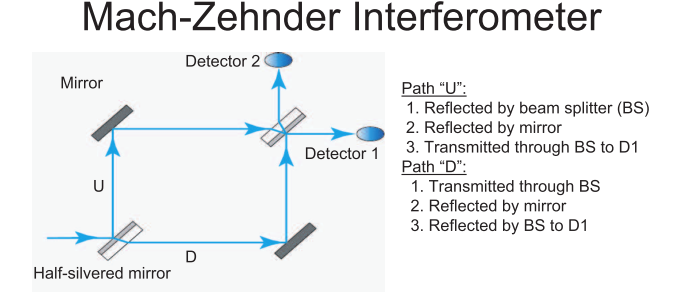
\includegraphics[scale=0.5]{Figures/mach-zender.png}
\caption{The Mach-Zehnder interferometer}
\label{mach-zehnder}
\end{figure}

As reflection results in a phase shift of $\pi$ and assuming transmission through the half-mirrors results in a phase shift of $\delta$ we easily calculate the phase differences of the two paths at the two detectors. At detector 1 and path $U$ there is a total of two reflections and a single transmission which results in a phase shift of $2\pi+\delta$. Similarly for path $D$ the phase shift is also $2\pi + \delta$. therefore at detector 1 there is constructive interference. At detector 2 path $U$ has a phase of $2\pi + 2\delta$ and path $D$ has a phase of $\pi + 2\delta$. Therefore at detector 2 there is destructive interference.\cite{dimaThesis}



\subsection{Bragg Scattering}
In neutron interferometry the crystal planes of the interferometer blades act as diffraction gratings. Incident waves that satisfy the Bragg condition \ref{bragg} are coherently scattered.
\begin{equation}
\label{bragg}
n\lambda = 2d sin(\theta_{b})
\end{equation} 
Where $n$ is a positive integer, $d$ is the distance between the atomic planes of the crystal lattice and $\theta_{b}$ is the angle between the incident beam and the atomic plane of the crystal. The amplitudes of the transmitted and the reflected beams are given by the coefficients $t$ (transmitted) and $r$ reflected.\cite{dimaThesis} 


